\documentclass[letterpaper,10pt]{article}
\usepackage{graphicx}
\usepackage[margin=2cm]{geometry}
\usepackage{url}
\usepackage{listings}

\title{Guided Programming: Creating a Producer}
\author{44-671: Streaming Data}
\date{}

\begin{document}
\maketitle

Note: In my experience the Docker application remembers my files between starts and stops, but I cannot guarantee that behavior.
If you do not intend on finishing this assignment in a single sitting I recommend downloading your producer notebook (by right clicking on it) just in case it does not persist when you stop your Docker application.

\begin{enumerate}
	\item Start your Docker application you set up in the Software Installation assignment
	\item Open a web browser and open JupyterLab (\url{http://localhost:8888/lab})
	\item Using the ``upload'' button (highlighted in yellow in the image below), upload the following files:
		\begin{center}
			
\includegraphics{upload-btn.PNG}
		\end{center}
		\begin{itemize}
			\item \texttt{d3.v4.min.js}
			\item \texttt{d3consumer.ipynb}
		\end{itemize}
	\item Open \texttt{d3consumer.ipynb} and change the name of the RabbitMQ instance to what your instance is called.
	\item Create a new Python Notebook named \texttt{yourname-producer.ipynb} (replace \texttt{yourname} with your name; you can right click on the file in the left pane to rename the file)
	\item Create two new cells in your notebook, and write the following code (replace the RabbitMQ instance with your instance name).  Use the new cell button to create the cells; don't run the cells just yet:
		\begin{center}
			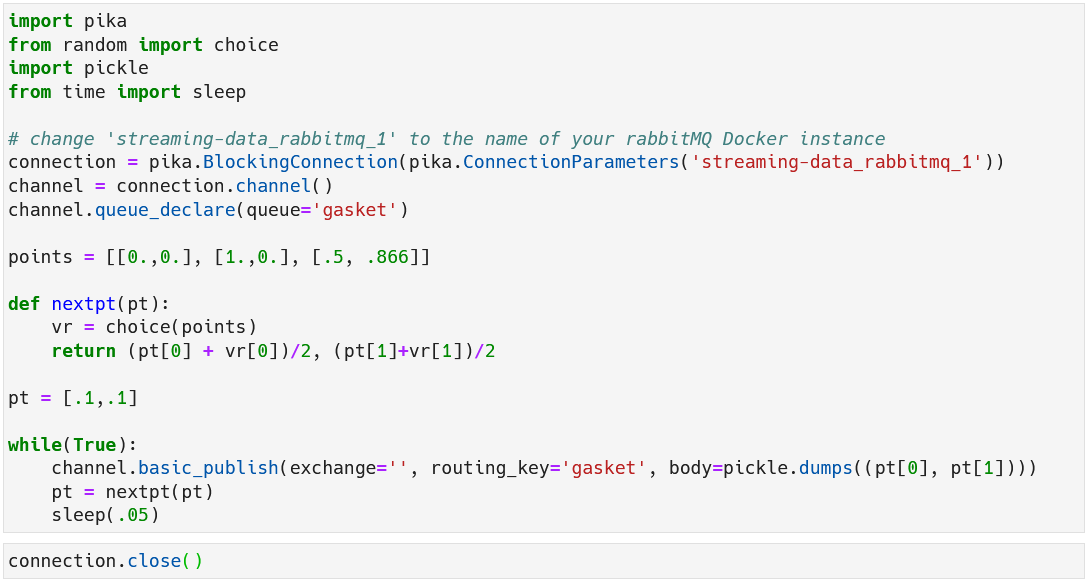
\includegraphics[width=0.9\textwidth]{producer-code.PNG}
		\end{center}
	\item Start the consumer; in \texttt{d3consumer.ipynb} select the second code cell (that starts with the comment \texttt{\#Run this cell}) and run it (either with the run button or Ctrl + Enter).  Make sure you see a \texttt{[*]} next to the cell; no output should appear yet.  If you encounter errors you probably need to fix the RabbitMQ instance name; if there are other errors contact your instructor for help debugging.
	\item Once your consumer is running, go back to your other notebook and start your first code cell; there should be no errors; if there are, fix them as above.
	\item Go back to the \texttt{d3consumer.ipynb} notebook; You should notice the plot above the consumer code changing.
	\item Let your code run for a while; you should see a shape start to appear.  Once the shape starts solidify, take a screenshot of the shape.
	\item Stop the code by doing the following steps in order:
		\begin{enumerate}
			\item Open your producer notebook and hit the ``stop'' button (the square) that is above the notebook (you should see an ``error'' that says \texttt{Keyboard Interrupt}).
			\item Run the second code cell (that contains \texttt{connection.close()})
			\item Open the \texttt{d3consumer.ipynb} notebook and hit the stop button.
			\item Run the code cell that contains \texttt{connection.close()}
		\end{enumerate}
	\item Add a new cell to the bottom of your producer notebook; in the dropdown box above the notebook that says ``Code'', select ``Markdown'', and answer the following questions (if you want to format the questions nicely, you can find a good Markdown tutorial at \url{https://www.markdowntutorial.com/} and a reference at \url{https://guides.github.com/features/mastering-markdown/}):
		\begin{itemize}
			\item Your producer was generating $(x,y)$ coordinates that the consumer was plotting; what shape was being create? Hint: you may want to search for the term ``chaos game''
			\item The first code cell in the producer notebook is what generates the points and adds them to the RabbitMQ; what lines of code would you need to modify to access a live source of data (such as access logs or social media) instead of modifying and generating points?
			\item Based on your reading and any understanding of the code you may have, if you wrote another producer that wrote to a different queue, would our consumer take that data?
			\item What do you think would happen if we started another producer writing to the same queue?
		\end{itemize}
	\item ``Run'' your Markdown cell (so it formats nicely)
\end{enumerate}
When you are finished, save your notebook and export it as a PDF. Submit both your PDF and screen shot of the shape that was created to the assignment on the course website.
You can stop your Docker application while you are not using it to save resources on your computer.
\end{document}
